\section{Introduction}
\label{fr:sec:introduction}
\subsection{Contexte}
La complexité grandissante des fonctionnalités embarquées dans les avions et l'obsolescence
progressive des processeurs mono-c\oe{}ur dans le commerce entrainent un besoin croissant
vers l'adoption de processeurs multi-c\oe{}urs dans les syst\`emes aéronautiques.
Or pour voler, un avion doit passer la certification, ce qui signifie
qu'un avionneur postulant -- que nous appellerons dans la suite un \emph{applicant} --
doit pr\'esenter un dossier argumentant que le système dans son ensemble est conforme \`a la
règlementation en vigueur.
Le cas des multi-c\oe{}urs est assez spécial et nouveau car un nouveau standard a vu le jour récemment
le CAST-32A (\cite{cast32}). Ce document est focalisé sur les particularités propres aux processeurs
multi-c\oe{}urs.
Cette th\`ese  a été financée par le  projet Phylog \cite{erts18}, dont 
l'objectif est de fournir à l'applicant une méthodologie outillée lui permettant
de préparer un dossier de certification pour des syst\`emes s'exécutant sur des cibles multi-c\oe{}urs
et donc de répondre au CAST-32A.
Parmi les objectifs du CAST32-A, le \textit{Resource Usage 3 (RU3)} nous intéresse particulièrement dans cette thèse.
En effet, RU3  correspond
au fait que l'applicant a identifié les canaux d'interférence qui pourraient
affecter les applications hébergées sur les c\oe{}urs et qu'il a
validé sa stratégie  pour en atténuer les effets nocifs.
Afin d'aider l'applicant à remplir cet objectif, cette thèse se concentre sur les
interférences
générées par \emph{la cohérence de cache}.

\begin{definition}[Interférence]
Une interférence est une modification indésirable du temps d'exécution d'une
application  provoquée par les actions d'une autre s'exécutant sur un c\oe{}ur distant.
\end{definition}

Afin de répondre à \textit{RU3}, l'applicant doit identifier
les sources d'interférence et quantifier leur impact sur les applications. Cela nécessite
une bonne compréhension des mécanismes présents sur l'architecture choisie.
Idéalement, la solution serait de simplement consulter la documentation
du processeur, où tous les mécanismes seraient décrits en détails, ainsi que
tous les comportements qui induiraient de l'interférence. Cependant, la
documentation des processeurs COTS n'inclut généralement pas de détails sur
la cohérence de cache. C'est donc une première problématique adressée par cette
thèse. Une fois cette étape d'identification menée, il faut comprendre les effets des interférences.

\begin{definition}[Impact associé à une interférence]
\label{fr:sec:impact_of_interference}
L'impact d'une interférence est une quantification des effets temporels sur l'exécution d'une application. Plus précisément, il s'agit de
la quantité de cycles processeur requis pour l'exécution d'un fragment de
l'application avec des autres applications s'exécutant en parallèle
comparée à son exécution en isolation.
\end{definition}

Prédire l'impact d'une interférence sur l'exécution des programmes
n'est pas simple et il n'existe à ce jour aucune méthodologie pour répondre à cette question.
La littérature propose soit des stratégies d'analyse très pessimistes ou
soit des restrictions pour l'élimination des sources d'interférence
pour ne pas à avoir à prendre leurs effets en compte.
De plus aucune analyse ne prend en charge la cohérence de cache.


\subsection{Contributions}
Cette thèse porte sur l'identification des interférences générées par les
mécanismes de cohérence de caches ainsi que sur les moyens de prédiction de
leurs effets sur les applications en vue de réduire les effets négatifs temporels.
Seules les architectures COTS avec cohérence de cache sont considérées.
De plus, parmi les protocoles de cohérence de cache,
nous nous concentrons sur ceux dits \emph{snooping} car les plus répandus dans les architectures.
D'autres restrictions ont été supposées dans le cadre de la thèse: pas de hiérarchie de cache, un cache local par c\oe ur, politique de placement associative et politique de remplacement LRU.
Un exemple d'architecture est montrée par la
Figure~\ref{fr:fig:second_intro:typical_arch}.

\begin{figure}[hbt]
\begin{center}
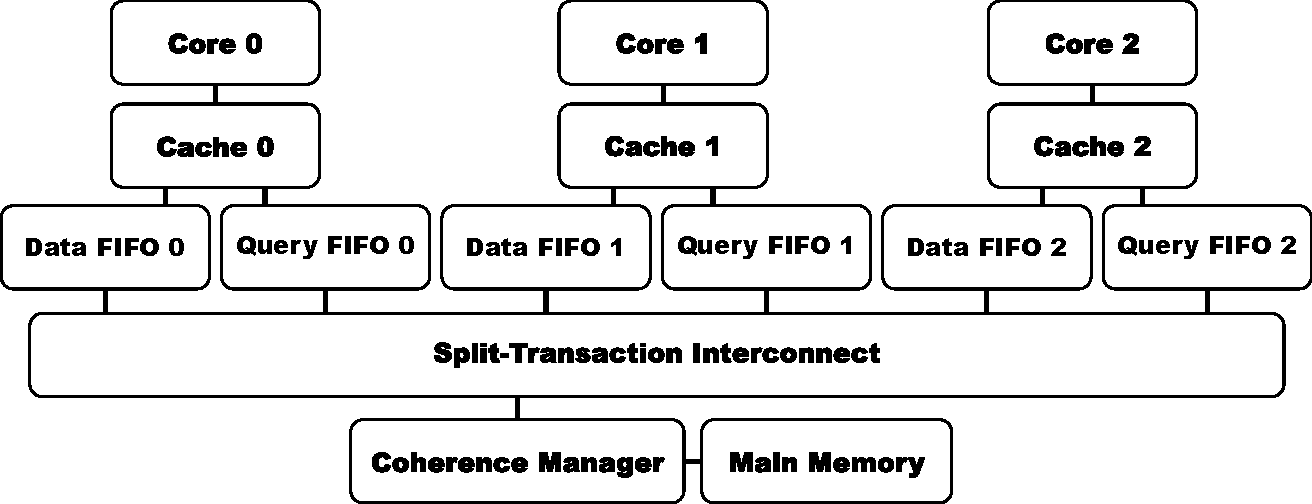
\includegraphics[width=.75\textwidth]{\chapterdirectory/figure/typical_arch3.pdf}
\end{center}
\caption{Profil typique d'architecture visée}
\label{fr:fig:second_intro:typical_arch}
\end{figure}

L'objectif de la thèse est de définir une méthodologie outillée
de compréhension et analyse des 
interférences générées par la cohérence de cache sur
une architecture
multi-c\oe{}ur COTS.
La Figure~\ref{fr:fig:second_intro:approach} présente le framework
proposé.


\begin{figure}[hbt]
\iffalse
\begin{subfigure}[t]{\textwidth}
\centering
\begin{tikzpicture}[
  font=\sffamily,
  every matrix/.style={ampersand replacement=\&,column sep=2.5cm,row sep=1cm},
  source/.style={draw,thick,rounded corners,fill=yellow!20,inner sep=.3cm},
  process/.style={draw,thick,circle,fill=blue!20},
  sink/.style={source,fill=green!20},
  datastore/.style={draw,very thick,shape=datastore,inner sep=.3cm},
  dots/.style={gray,scale=2},
  to/.style={->,>=stealth',shorten >=1pt,semithick,font=\sffamily\footnotesize},
  every node/.style={align=center}]

  % Position the nodes using a matrix layout
  \matrix{
    \node[datastore] (architecture) {Architecture};
      \& \node[sink] (identification) {%
         \begin{tabular}{@{}c@{}}
            Cache Coherence Identification\\
            (Chapter~\ref{cha:identifying_cache_coherence})
         \end{tabular}
         };
      \&
    \node[datastore] (cacheprotocol) {%
         \begin{tabular}{@{}c@{}}
            Cache Coherence\\ Protocol
         \end{tabular}
         };
      \\
  };

  % Draw the arrows between the nodes and label them.
  \draw[to] (architecture) to (identification);

  \draw[to] (identification) to (cacheprotocol);
\end{tikzpicture}

\end{subfigure}
\begin{subfigure}[t]{\textwidth}
\vspace{2em}
\centering
\begin{tikzpicture}[
  font=\sffamily,
  every matrix/.style={ampersand replacement=\&,column sep=2.5cm,row sep=1cm},
  source/.style={draw,thick,rounded corners,fill=yellow!20,inner sep=.3cm},
  process/.style={draw,thick,circle,fill=blue!20},
  sink/.style={source,fill=green!20},
  datastore/.style={draw,very thick,shape=datastore,inner sep=.3cm},
  dots/.style={gray,scale=2},
  to/.style={->,>=stealth',shorten >=1pt,semithick,font=\sffamily\footnotesize},
  every node/.style={align=center}]

  % Position the nodes using a matrix layout
  \matrix{
   \&
    \node[datastore] (cacheprotocol) {%
         \begin{tabular}{@{}c@{}}
            Cache Coherence\\ Protocol
         \end{tabular}
         };
      \&
   \\
    \node[datastore] (architecture) {Architecture};
      \&
      \node[source] (benchmarking) {%
         \begin{tabular}{@{}c@{}}
            Benchmarking\\
            (Chapter~\ref{cha:micro-benchs})
         \end{tabular}
      };
      \&
    \node[datastore] (cacheperformance) {%
         \begin{tabular}{@{}c@{}}
            Cache Coherence\\
            Performance
         \end{tabular}
      };
      \\
  };

  % Draw the arrows between the nodes and label them.
  \draw[to] (architecture) to (benchmarking);
  \draw[to] (cacheprotocol) to (benchmarking);

  \draw[to] (benchmarking) to (cacheperformance);
\end{tikzpicture}

\end{subfigure}
\begin{subfigure}[t]{\textwidth}
\vspace{4em}
\centering
\begin{tikzpicture}[
  font=\sffamily,
  every matrix/.style={ampersand replacement=\&,column sep=2.5cm,row sep=1cm},
  source/.style={draw,thick,rounded corners,fill=yellow!20,inner sep=.3cm},
  process/.style={draw,thick,circle,fill=blue!20},
  sink/.style={source,fill=green!20},
  datastore/.style={draw,very thick,shape=datastore,inner sep=.3cm},
  dots/.style={gray,scale=2},
  to/.style={->,>=stealth',shorten >=1pt,semithick,font=\sffamily\footnotesize},
  every node/.style={align=center}]

  % Position the nodes using a matrix layout
  \matrix{
   \node[datastore] (application) {Application};
   \&
    \node[datastore] (cacheprotocol) {%
         \begin{tabular}{@{}c@{}}
            Cache Coherence\\ Protocol
         \end{tabular}
         };
      \&
   \\
      \&
      \node[sink] (uppaal) {
         \begin{tabular}{@{}c@{}}
            UPPAAL Analysis\\
            (Chapters~\ref{cha:modeling_cache_coherence} and
            \ref{chap:exposing_interference})
         \end{tabular}
         };
      \&
      \node[datastore] (coherenceeffect) {%
         \begin{tabular}{@{}c@{}}
            Cache Coherence\\
            Impact
         \end{tabular}
      };
      \\
    \node[datastore] (architecture) {Architecture};
    \& \node[datastore] (cacheperformance) {%
         \begin{tabular}{@{}c@{}}
            Cache Coherence\\
            Performance
         \end{tabular}
      };
   \\
  };

  % Draw the arrows between the nodes and label them.

  \draw[to] (architecture) to (uppaal);
  \draw[to] (cacheperformance) to (uppaal);
  \draw[to] (cacheprotocol) to (uppaal);
  \draw[to] (application) to (uppaal);

  \draw[to] (uppaal) to (coherenceeffect);
\end{tikzpicture}

\end{subfigure}
\fi
\centering
\begin{tikzpicture}[
  font=\sffamily,
  every matrix/.style={ampersand replacement=\&,column sep=2.5cm,row sep=1cm},
  source/.style={draw,thick,rounded corners,fill=yellow!20,inner sep=.3cm},
  process/.style={draw,thick,circle,fill=blue!20},
  sink/.style={source,fill=green!20},
  datastore/.style={draw,very thick,shape=datastore,inner sep=.3cm},
  dots/.style={gray,scale=2},
  to/.style={->,>=stealth',shorten >=1pt,semithick,font=\sffamily\footnotesize},
  every node/.style={align=center}]

  % Position the nodes using a matrix layout
  \matrix{
    \node[datastore] (architecture) {Architecture};
      \& \node[sink] (identification) {%
         \begin{tabular}{@{}c@{}}
            Cache Coherence Identification\\
            (Chapter~\ref{cha:identifying_cache_coherence})
         \end{tabular}
         };
      \&
    \node[datastore] (cacheprotocol) {%
         \begin{tabular}{@{}c@{}}
            Cache Coherence\\ Protocol
         \end{tabular}
         };
      \\


   \&
      \&
   \\
      \&
      \node[source] (benchmarking) {%
         \begin{tabular}{@{}c@{}}
            Benchmarking\\
            (Chapter~\ref{cha:micro-benchs})
         \end{tabular}
      };
      \&
    \node[datastore] (cacheperformance) {%
         \begin{tabular}{@{}c@{}}
            Cache Coherence\\
            Performance
         \end{tabular}
      };
      \\



   \&
      \&
   \\
      \node[datastore] (application) {Application};
      \&
      \node[sink] (uppaal) {
         \begin{tabular}{@{}c@{}}
            UPPAAL Analysis\\
            (Chapters~\ref{cha:modeling_cache_coherence} and
            \ref{chap:exposing_interference})
         \end{tabular}
         };
      \&
      \node[datastore] (coherenceeffect) {%
         \begin{tabular}{@{}c@{}}
            Cache Coherence\\
            Impact
         \end{tabular}
      };
   \\
  };

  % Draw the arrows between the nodes and label them.
  \draw[to] (architecture) to (identification);

  \draw[to] (identification) to (cacheprotocol);



  \draw[to] (architecture) to (benchmarking.north west);
  \draw[to] (cacheprotocol) to (benchmarking.north east);

  \draw[to] (benchmarking) to (cacheperformance);



  \draw[to] (architecture) to (uppaal.north west);
  \draw[to] (cacheperformance) to (uppaal.north east);
  \draw[to] (cacheprotocol) to (uppaal);
  \draw[to] (application) to (uppaal);

  \draw[to] (uppaal) to (coherenceeffect);
\end{tikzpicture}

\caption{Vue d'ensemble de l'approche}
\label{fr:fig:second_intro:approach}
\end{figure}

La première contribution adresse les ambiguïtés dans la compréhension que les applicants
ont de la cohérence de cache réellement présente dans l'architecture.
En effet, la documentation des architectures
ne fournit généralement pas suffisamment de détails sur les protocoles.
Cette thèse propose une formalisation des protocoles standards,
ainsi qu'une stratégie, reposant sur les micro-benchmarks,
pour clarifier les choix d'implémentation du protocole de
cohérence présent sur l'architecture. Cette stratégie a notamment été appliquée sur le NXP
QorIQ T4240.

Une fois le protocole correctement identifié, les techniques existantes de
mesure de performance peuvent être appliquées afin d'obtenir des
informations sur la performance des mécanismes de cohérence de cache identifiés.
Cela ne constitue pas une contribution, d'où la coloration différente de cette
étape dans la Figure~\ref{fr:fig:second_intro:approach}.

La seconde
contribution consiste à réaliser une description bas-niveau de l'architecture
en utilisant des automates temporisés afin de représenter convenablement les
micro-comportements et comprendre clairement comment le protocole de cohérence
de cache agit. Ainsi, un framework de génération de modèles génériques a été
développé, capable de supporter plusieurs protocoles de cohérence de cache et de représenter différents agencements d'architectures
afin de mieux correspondre à l'architecture choisie par l'applicant.

La
troisième contribution explique comment utiliser cette représentation de
l'architecture pour exhiber les interférences. Elle propose une stratégie pour
détailler les causes et effets de chaque interférence liée à la cohérence de caches
sur les programmes.
Commençant par une simple analyse de temps d'exécution, les résultats
descendent jusqu'au niveau des instructions pour indiquer comment chaque
instruction génère et souffre des interférences. L'objectif étant alors de
fournir suffisamment d'information à l'applicant à la fois pour la certification, mais aussi pour définir une
stratégie d'atténuation et de maîtrise des effets temporels.

\subsection{Vue d'ensemble du r\'esum\'e}
Ce résumé  commence par les préliminaires nécessaires à la
compréhension de la problématique et des solutions proposées: les automates
temporis\'es (Section~\ref{fr:sec:formal_methods}) et la cohérence de cache
(Section~\ref{fr:sec:cache_coherence}). Une fois ces notions 
présentées, le résumé présentera rapidement l'état de l'art (Section~\ref{fr:sec:rel_works}).

Les trois contributions apportées
par cette thèse sont ensuite détaillées: une stratégie d'identification détaillée du protocole de cache
utilisé par l'architecture 
(Section~\ref{fr:sec:identify}); un template de modèle d'architecture
multi-c\oe{}urs supportant la cohérence de cache (Section~\ref{fr:sec:model});
et les analyses à faire sur les modèles instanciés afin déterminer les causes
et effets des interférences (Section~\ref{fr:sec:analyze}).
